% Digital Logic Report Template
% Created: 2020-01-10, John Miller

%==========================================================
%=========== Document Setup  ==============================

% Formatting defined by class file
\documentclass[11pt]{article}

% ---- Document formatting ----
\usepackage[margin=1in]{geometry}	% Narrower margins
\usepackage{booktabs}				% Nice formatting of tables
\usepackage{graphicx}				% Ability to include graphics

%\setlength\parindent{0pt}	% Do not indent first line of paragraphs 
\usepackage[parfill]{parskip}		% Line space b/w paragraphs
%	parfill option prevents last line of pgrph from being fully justified

% Parskip package adds too much space around titles, fix with this
\RequirePackage{titlesec}
\titlespacing\section{0pt}{8pt plus 4pt minus 2pt}{3pt plus 2pt minus 2pt}
\titlespacing\subsection{0pt}{4pt plus 4pt minus 2pt}{-2pt plus 2pt minus 2pt}
\titlespacing\subsubsection{0pt}{2pt plus 4pt minus 2pt}{-6pt plus 2pt minus 2pt}

% ---- Hyperlinks ----
\usepackage[colorlinks=true,urlcolor=blue]{hyperref}	% For URL's. Automatically links internal references.

% ---- Code listings ----
\usepackage{listings} 					% Nice code layout and inclusion
\usepackage[usenames,dvipsnames]{xcolor}	% Colors (needs to be defined before using colors)

% Define custom colors for listings
\definecolor{listinggray}{gray}{0.98}		% Listings background color
\definecolor{rulegray}{gray}{0.7}			% Listings rule/frame color

% Style for Verilog
\lstdefinestyle{Verilog}{
	language=Verilog,					% Verilog
	backgroundcolor=\color{listinggray},	% light gray background
	rulecolor=\color{blue}, 			% blue frame lines
	frame=tb,							% lines above & below
	linewidth=\columnwidth, 			% set line width
	basicstyle=\small\ttfamily,	% basic font style that is used for the code	
	breaklines=true, 					% allow breaking across columns/pages
	tabsize=3,							% set tab size
	commentstyle=\color{gray},	% comments in italic 
	stringstyle=\upshape,				% strings are printed in normal font
	showspaces=false,					% don't underscore spaces
}

% How to use: \Verilog[listing_options]{file}
\newcommand{\Verilog}[2][]{%
	\lstinputlisting[style=Verilog,#1]{#2}
}




%======================================================
%=========== Body  ====================================
\begin{document}

\title{ELC 2137 Lab \11: FSM: Guessing Game}
\author{Spencer Stinson}

\maketitle


\section*{Summary}

In this lab, we learned how to use state diagrams as a guideline to write a source code in Verilog. Doing this helped us to show our knowledge of both how state diagrams work, as well as how verliog works as we integrated the two together. We used moore machine design to implement this and it allowed us to create this game. By applying the knowldge we learned in class, we helped to make ourselves remember this, and to figure out the things that we may not have known in its entirety. 


\section*{Q\&A}

\begin{itemize}
	\item At what time in the simulation did the debounce circuit reach each of the four state? (zero, wait1, one, wait0)
	In my simulation, the values for the zero is from 0-40 ns, for wait1 is from 220-420, for one is from 600-620, for wait 0 from 620-800.
\end{itemize}
\begin{itemize}
	\item Why can this game not be implemented with regular sequential logic?
	Regular sequential logic cannot be used because many of these need to happen simultaneously, and state changes will happen too many times if we use sequential logic. 
\end{itemize}
\begin{itemize}
	\item What type of outputs did you use for your design(Mealy or Moore)?
	This machine is a Moore machine becuase the output depends on the state. 
\section*{Results}
\begin{figure}
	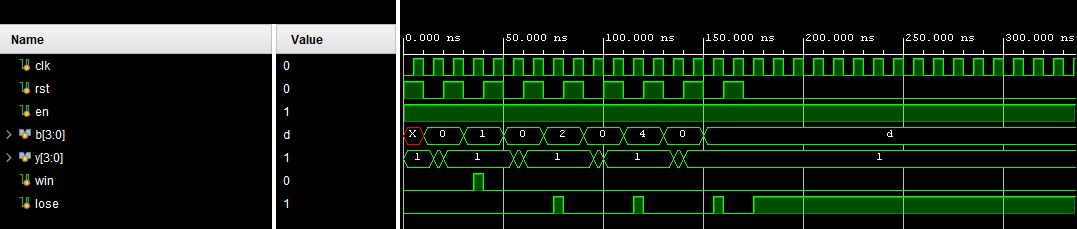
\includegraphics[width=\textwidth]{waveform1.png}
	\caption{Guess FSM waveform}
	\label{fig: gfw}
\end{figure}
\begin{figure}
	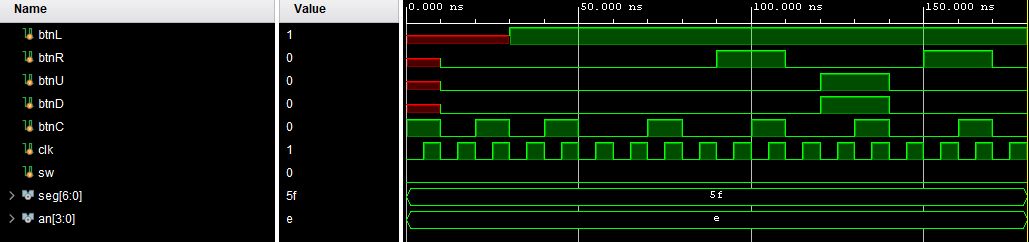
\includegraphics[width=\textwidth]{waveformgame.png}
	\caption{Guessing game waveform}
	\label{fig: ggw}
\end{figure}
\begin{figure}
	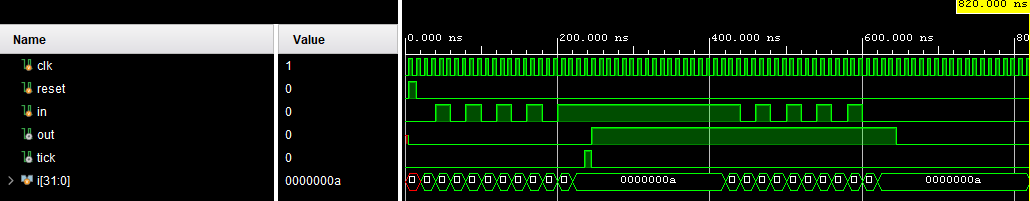
\includegraphics[width=\textwidth]{debouncewaveform.png}
	\caption{Debounce waveform}
	\label{fig: ggw}
\end{figure}
\begin{figure}
	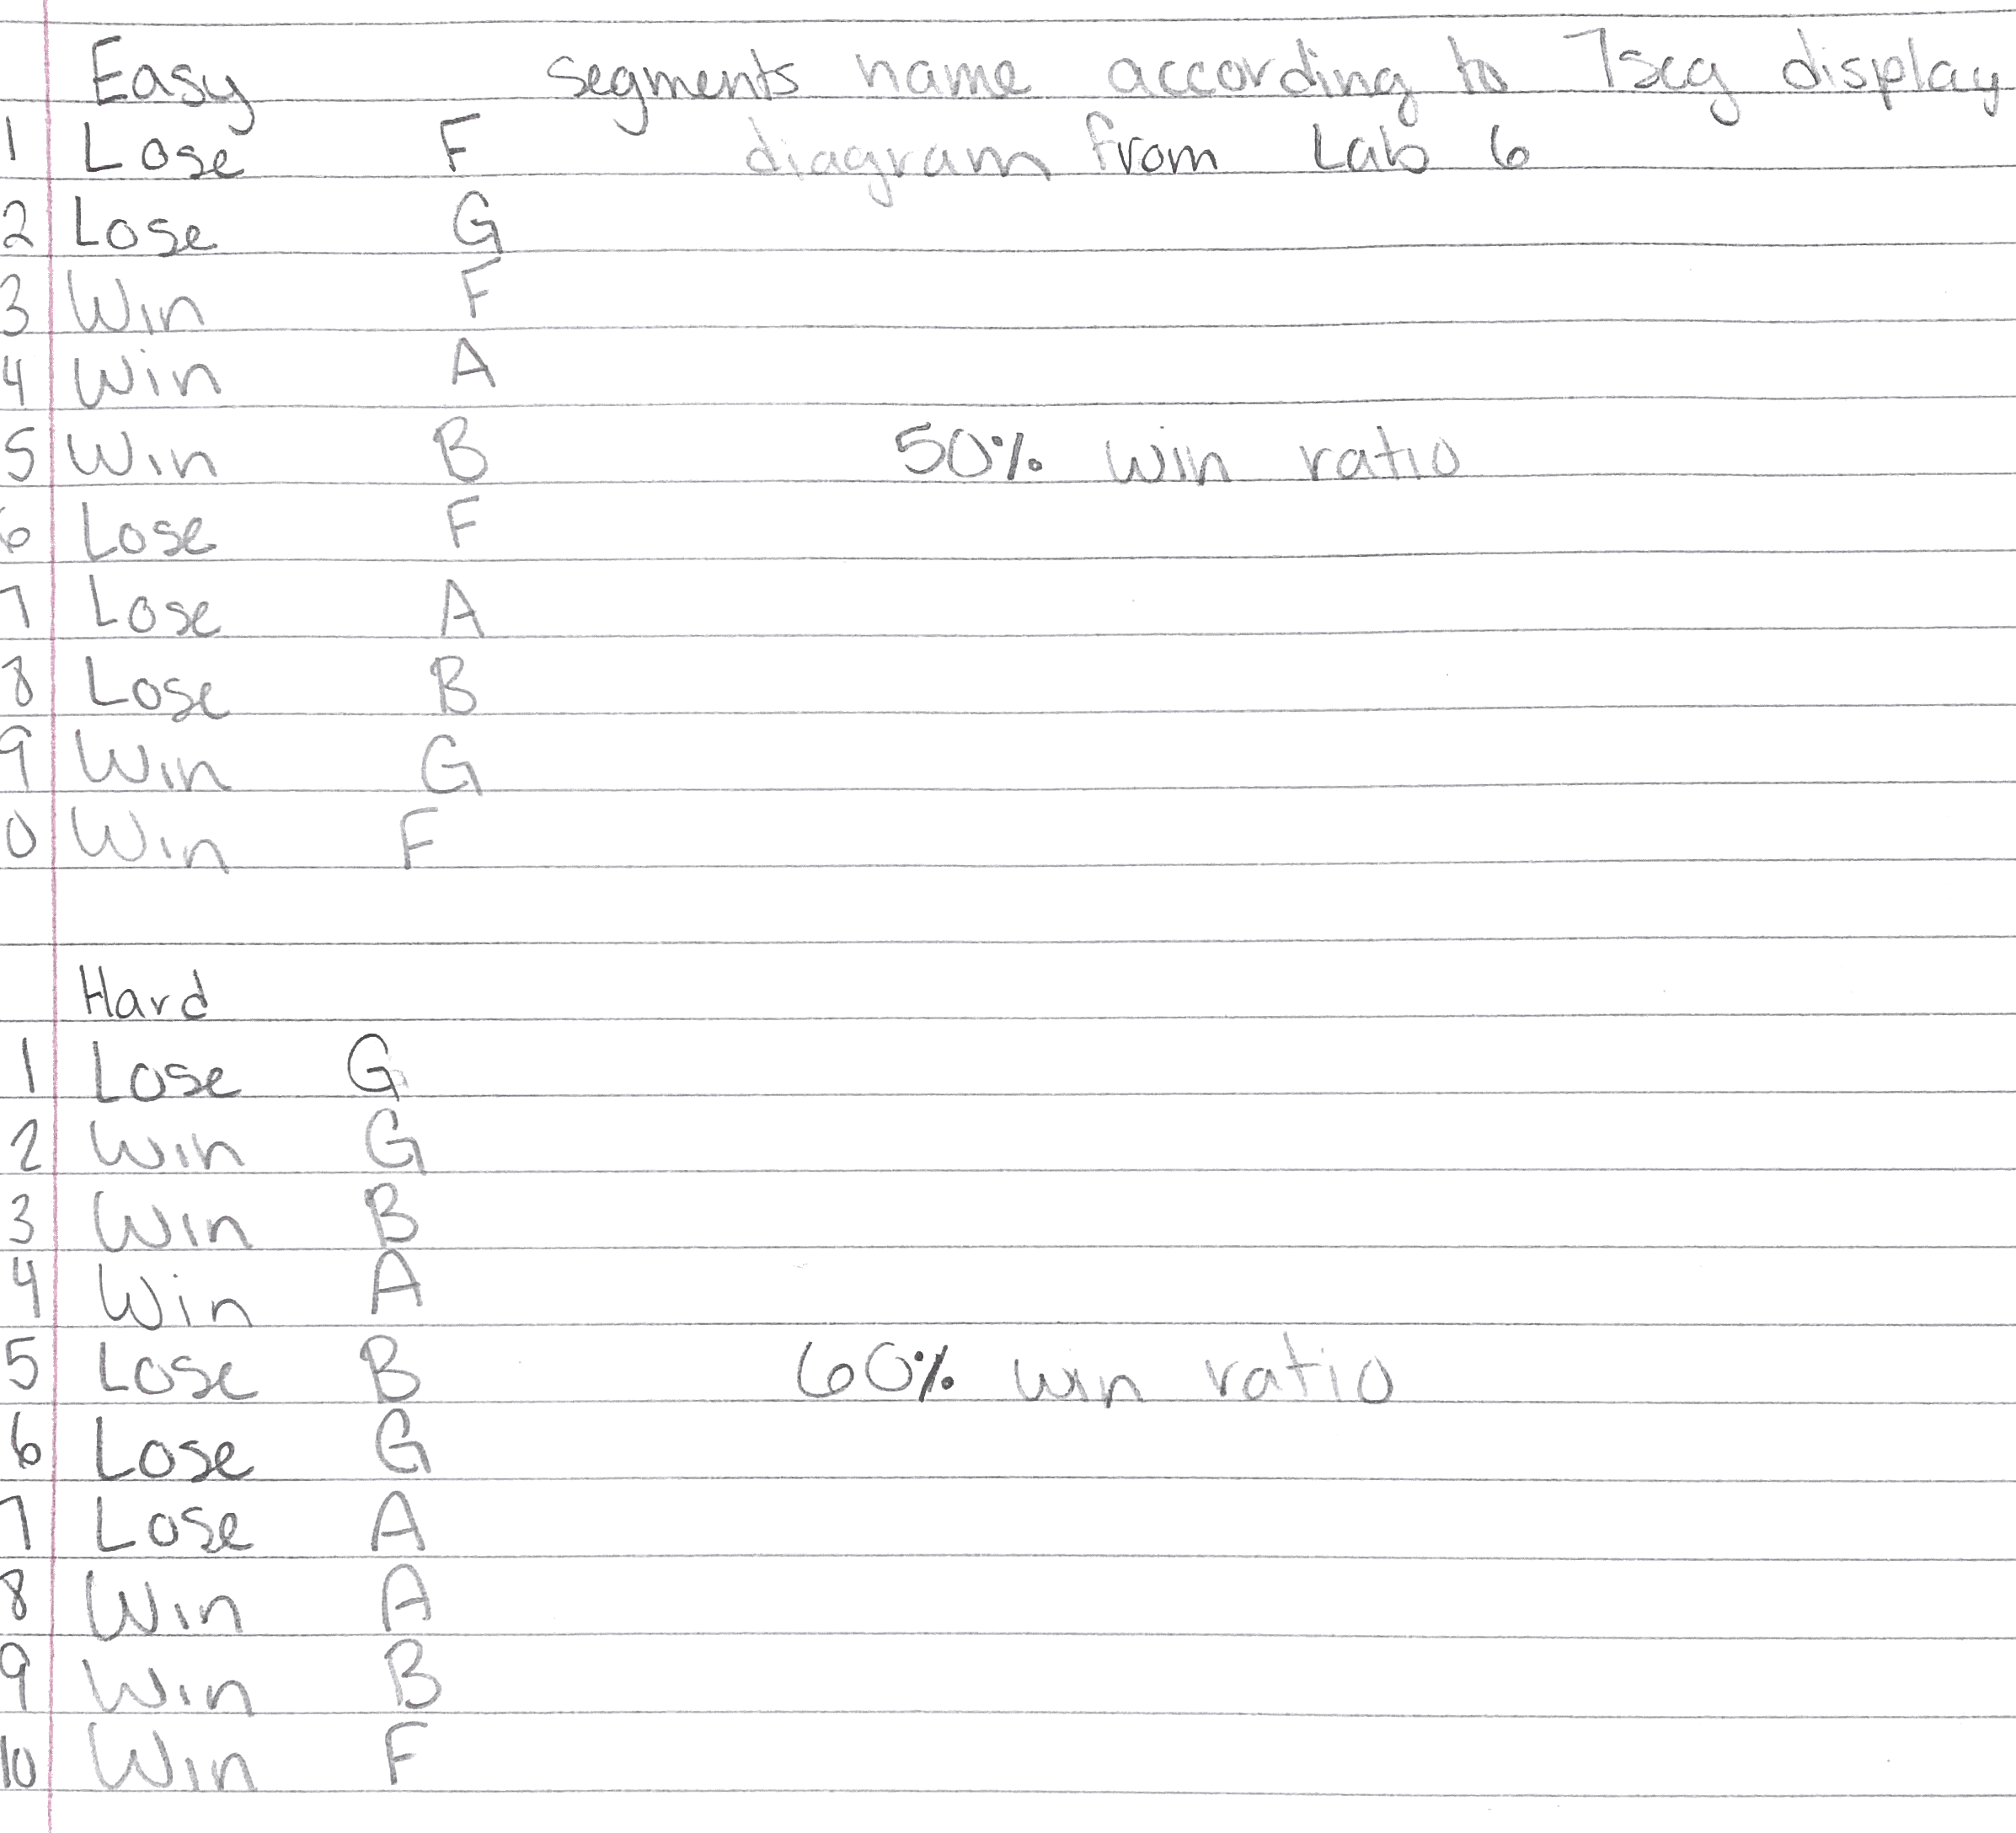
\includegraphics[width=\textwidth]{gameresults.png}
	\caption{Game results table}
	\label{fig:grt}
\end{figure}

\section*{Code}

\Verilog[caption= Counter module]{C:/Users/spencer_stinson1/Documents/GitHub/Lab11/Lab_11/Lab_11.srcs/sources_1/new/counter.sv}
\Verilog[caption= Display setup module]{C:/Users/spencer_stinson1/Documents/GitHub/Lab11/Lab_11/Lab_11.srcs/sources_1/new/sseg_game.sv}
\Verilog[caption= Guess FSM module]{C:/Users/spencer_stinson1/Documents/GitHub/Lab11/Lab_11/Lab_11.srcs/sources_1/new/guess_FSM.sv}
\Verilog[caption= Guessing game Module]{C:/Users/spencer_stinson1/Documents/GitHub/Lab11/Lab_11/Lab_11.srcs/sources_1/new/guessing_game.sv}
\Verilog[caption= Guess FSM testbench]{C:/Users/spencer_stinson1/Documents/GitHub/Lab11/Lab_11/Lab_11.srcs/sim_2/new/guess_FSM_test.sv}
\Verilog[caption= Game Testbench]{C:/Users/spencer_stinson1/Documents/GitHub/Lab11/Lab_11/Lab_11.srcs/sim_2/new/guess_FSM_test.sv}


\end{document}
